%SRS Document
%Copyright 2017 Yang LI
%https://github.com/zjzsliyang/42003201ObjectOrientedAnalysisAndDesign
%Under GPL-3.0 License

\documentclass[12pt]{scrreprt}
\usepackage{outline}
\usepackage{pmgraph}
\usepackage[normalem]{ulem}
\usepackage{graphicx}
\usepackage{verbatim}
\usepackage{hyperref}
\usepackage{color}
\usepackage{setspace}
\title{

\includegraphics[width=0.8in]{DocumentRes/OnionExpress.png} \\
\vspace*{1in}
\textbf{Software Requirements Specification}}
\author{Yang LI\\
        Zhongjin LUO\\
        Guohui YANG\\
        Yirui WANG\\
        Xinying WU\\
        Yiqun LIN\\
		    \vspace*{0.5in} \\
		    School of Software Engineering\\
        \textbf{Tongji University}\\
        Group 4\\
}
\date{\today}

\setlength{\oddsidemargin}{0in}
\setlength{\evensidemargin}{0in}
\setlength{\topmargin}{0in}
\setlength{\headsep}{-.25in}
\setlength{\textwidth}{6.5in}
\setlength{\textheight}{8.5in}
\setlength{\parindent}{1cm}

\begin{document}
\maketitle
\tableofcontents

\chapter{Introduction}
Onion Express\textregistered\ is a system built for logistic companies,
which provides them with a solution to logistics tracking, goods packing,
goods distribution, after-sales management, data storage, information
processing, etc.

\section{Purpose}
These days as B2C business is increasing rapidly, the growth of
logistics business is also remarkable. The enormous market demand
brings logistics companies opportunities as well as the challenge.
Facing such kind of condition, this project is aimed at improving the
efficiency of field personnel and customer satisfaction of a logistics
company by building a cross-platform system.

\section{Definitions}
As Jobs has ever said, “People don't know what I really want at all,
until your products are in their eyes”. This project is specially
designed for an independent logistics companies like UPS. The business
scope is limited within China. To be more precise, the express is only
available in Jiangsu, Zhejiang and Shanghai at the beginning.
Temporarily private orders are not covered in the business scope,
which means the express company corporates with e-commercial companies only
with the cash-on-delivery express or normal express. The system focuses on logistics
service without regard to O2O, bulk cargo or self-support e-business.
Timing express might be expanded in future.

\section{System Overview}
The actors in the system are classified as \emph{Postman, E-business, Customer
service, Customer} and \emph{Agent}. \emph{Customer} and \emph{Agent} are
generalized as Receiver. The \emph{Postman} has access to this system
only on mobile devices while \emph{Customer} has access both on browsers
as well as mobile devices. \emph{E-business} offers orders periodically.
\emph{Customer service} helps to deal with tasks cannot be done only by
the system.\\
Web application and iOS application provide different functions for different
users to enhance user experience and have some humanization design(e.g.
using different colors to mark tasks as reception or delivery in postman’s app).
Besides basic functions, the system also provides some advanced functions,
like printing invoices. Different offline payment methods are supported.
And the customer’s telephone number is hidden to protect his/her privacy.\\
The postman is equipped with a multifunctional special device, when the
customer receives his/her package, he/she can use this device to pay by
card and can also press thumb on it to sign digitally, besides, the device
helps collect postman’s GPS location accurately.\\
The system considers all the 8 scenarios, including sending the package,
paying for the product, signing the package and so on. To integrate the
system, two scenarios are added. One is creating the orders, at the beginning
of the entire flow. Another is dealing the order manually, to reduce errors
caused by the system and handle other unanticipated situations. That can
improve the stability of the system and in consideration of the relatively
small scale of users in the early stage, robot customer service is not
necessary. It can be taken into consideration when the business is expanding
to a certain stage.\\
This project also designs several user interface mock-ups on the website
and on mobile devices. Core functions are exhibited in these mock-ups,
for example, the dispatch list interface.\\
Nonfunctional requirements and further explanations on security, performance,
data storage and computing, tracking the package, maintenance and others are
detailed in supplementary Specification.

\chapter{Use Case Modelling}
\section{Activity Diagram}

\section{Use Case Diagram}
\subsection{Global Use Cases}
\begin{figure}[htbp]
  \centering
\includegraphics[width=3.5in]{DocumentRes/OnionExpress.png}
  \caption{Global Use Case Diagram}
\end{figure}
\subsection{Sub Use Cases}
\subsubsection{Payment View}

\subsubsection{Logistics Company View}

\subsection{Specification of Use Cases}
\subsubsection{Scenario 1}

\subsubsection{Scenario 2}

\subsubsection{Scenario 3}

\subsubsection{Scenario 4}

\subsubsection{Scenario 5}

\subsubsection{Scenario 6}

\subsubsection{Scenario 7}

\subsubsection{Scenario 8}


\chapter{Glossary of Terms}
\begin{spacing}{0.7}
\subsubsection{after-sales service}
Also called customer service, after sales service is the provision of
service to customers before, during and after a purchase.
\subsubsection{article}
The material in the package which is sent by a normal customer.
\subsubsection{bi-directional read}
The information can be read in both direction.
\subsubsection{cash-on-delivery express}
The sale of goods by express where payment is made on delivery rather
than in advance.
\subsubsection{claim}
When packages are damaged or lost, customers have right to ask for compensation.
\subsubsection{courier}
A courier is a person who delivers messages, packages, and mail. Here it refers
to postmen.
\subsubsection{customer service staff}
The staff in the logistics company serving customers.
\subsubsection{damaged express item}
The package that is damaged during express.
\subsubsection{decision support system(DSS)}
A decision support system is a computer-based information system that supports
 business or organizational decision-making activities.
\subsubsection{delivery}
A single task to send the package to a customer.
\subsubsection{delivery terminal}
The destination of the delivery where the receiver receive and sign the package.
\subsubsection{dispath list}
The digital list of information of the packages to be delivered in
postmen’s port.
\subsubsection{distribution center}
A station in a large district to transfer packages to the regional
distribution center.
\subsubsection{door-to-cfs}
From the shipper factory or warehouse to the destination or the
Container freight station of the discharging port.
\subsubsection{door-to-door}
From the shipper factory or warehouse to the consignee's factory
or warehouse.
\subsubsection{Electronic Data Interchange(EDI)}
Electronic Data Interchange is an electronic communication method that provides
standards for exchanging data via any electronic means.
\subsubsection{Electronic Order System(EOS)}
Electronic Order System is to meet demand instantly,
with perfect quality and punctuality.
\subsubsection{express item}
Packages to be delivered.
\subsubsection{express item tracking system}
A subsystem in our system to track the packages with GIS automatically.
\subsubsection{express network}
A service network within the scope to help delivery.
\subsubsection{express waybill}
An express receipt given by the carrier to the shipper acknowledging receipt
of the packages being shipped and specifying the terms of delivery.
\subsubsection{first time delivery}
The first time for particular postman to send the package to a position.
\subsubsection{Global Position System(GPS)}
The Global Positioning System is a space-based navigation system that
provides location and time information in all weather conditions,
anywhere on or near the Earth where there is an unobstructed line of
sight to four or more GPS satellites.
\subsubsection{Geographic Information System(GIS)}
A geographic information system is a system designed to capture,
store, manipulate, analyze, manage, and present all types of spatial
or geographical data.
\subsubsection{handheld terminal}
Handheld terminal refers to the portable data processing terminal
with some particular features. Here it refers to mobile phones with our app.
\subsubsection{inquiry}
The customer logins the system or connects with customer service staff to get
information about the order, operation instruction etc.
\subsubsection{Integrated Services Digital Network(ISDN)}
Integrated Services for Digital Network is a set of communication standards
for simultaneous digital transmission of voice, video, data, and other
network services over the traditional circuits of the public switched
telephone network.
\subsubsection{interchange receipt}
A voucher to certify that the customers or e-business commits articles
or products to the logistics company for delivery.
\subsubsection{Invoice(INV)}
An invoice is a commercial document issued by a seller to a buyer,
relating to a sale transaction and indicating the products, quantities,
and agreed prices for products or services the seller had provided the buyer.
\subsubsection{Just-in-time logistics(JIT logistics)}
Just-in-time logistics is a modern logistics method based on the JIT
management philosophy.
\subsubsection{lost express item}
The package that is lost during express.
\subsubsection{order number}
The number generalized when the order is created.
\subsubsection{order processing}
A series automatic operation in system to deal the order, such as
creating an order, completing an order and so on.
\subsubsection{package}
The material to be delivered after customers or the e-business company
create orders.
\subsubsection{product}
The material in the package which is ordered by customers from the
e-business company.
\subsubsection{QR code}
QR code (abbreviated from Quick Response Code) is the trademark for
a type of matrix barcode(or two-dimensional barcode) first designed for
the automotive industry in Japan.
\subsubsection{receiver}
Generalized from Customer and Agent, the person receiving and signing
the package directly.
\subsubsection{redelivery}
When no one can sign the package, the postman will carry it back to
the delivery terminal and the order will be rescheduled in the system.
\subsubsection{redirect express item}
When customer changes the destination or the destination is out of scope,
the package will be reassigned.
\subsubsection{regional distribution center}
The substation in a certain region of the logistics company to assign
packages to postmen.
\subsubsection{return}
If customers are unsatisfied with the product, he or she can send it back
with a label from system.
\subsubsection{sender}
The customer or the e-business company who sends the package.
\subsubsection{serial number of express}
i.e. the tracking number of packages in the system.
\subsubsection{sign in}
The receiver sign the package and get it.
\subsubsection{sorting}
The packages in the regional distribution center are sorted to transfer to
corresponding postmen or the packages in the distribution center are sorted to
transport to regional distribution centers.
\subsubsection{tracking number}
Especially for tracking the real-time GPS location of the package.
\subsubsection{withdrawal}
If the customer is unsatisfied with the product and has sent it back,
he or she can choose withdraw the order and the payment will be reimbursed.
\end{spacing}

\chapter{Supplementary Specification}
\section{Security}
The system should avoid the database being attacked and data being taken
advantage of by the wicked.
\subsection{Access and Data Integrity}
\begin{enumerate}
  \item The authorization of access to the system of postmen, customers
  and customer servers should be classified and announced clearly. With
  certain authorization, different users have limited access to data and
  operation.
  \item The server should use anti-virus software.
  \item Firewalls and network protection are necessary, and they should
  be updated in time.
  \item The atomic processes in the database will ensure the accuracy
  of the database.
\end{enumerate}

\subsection{Encryption}
\begin{enumerate}
  \item The session should not be transmitted in DNS.
  \item All texts and messages should be encrypted with Encryption Algorithm
  such as RSA, 3DES or IDEA.
  \item Two keys are used to identify a certain user. One public key is
  used for encryption and anther private key is used for decryption.
  The key is a completely random mix of letters.
  \item The session will record the activity of the customer, and if the
  customer has no operation for 5 minutes, he or she will log out the system
  automatically.
  \item After customers log out the system, all the private information(cookies)
  will be cleaned.
\end{enumerate}

\subsection{Digital Certificates}
\begin{enumerate}
  \item We use digital certificates as a replacement of user names and
  passwords, for example, SSL Certificates. It will be used automatically
  with the permission of users.
  \item The IP address or location where users log in the system will be
  recorded and when the account is used beyond their regular locations, the
  user will get alarmed.
\end{enumerate}

\subsection{Digital Signatures}
\begin{enumerate}
  \item Users should log in the system with a password. Our system will
  test its complexity. If it is too simple, the system will remind the
  users to complicate it. That involves cryptography.
  \item We use a message digest to ensure the integrality of the data.
  \item If necessary, we can extend our fingerprint system to login system.
\end{enumerate}

\section{Performance}
\begin{enumerate}
  \item The information of the package, including the real-time position,
  Order-ID, the postman etc., should be checked by customers in 3 seconds
  with at most 0.1\% error rate.
  \item The payment should be confirmed in 2 seconds by the system from
  the moment when the third party trade agent sends the message or the
  postmen report the payment.
  \item The order created by customers should be processed in 15 minutes.
  \item The orders obtained from e-business should be processed every
  hour(about 5,000 orders).
  \item Information of the delivery such as the phone number, the address,
  the receiver and others should be updated and checked by postman in 1 min.
  \item This system allows the e-business to create batch orders which can
  be sent at regular time.
  \item The estimate of delivery time should be accurate with the max
  uncertainty in 2 days.
  \item The expectation should be sent to custom service in 2 min from
  the time a postman reports it.
  \item This system’s unavailable time should be controlled in 20 minutes
  in a year.
  \item To offer the best user experience, a content delivery network
  should be used by this system.
\end{enumerate}

\section{Data Storage and Computing}
\begin{enumerate}
  \item To store a huge amount of data, distributed database should be used.
  And it should use Homogeneous Distributed Databases Management System.
  \item Considering that there may be an enormous number of visitors and
  inquiries at the same time, the system must implement cloud computing service.
  \item The system can support as many as 1500 times of visits per second.
  \item There must be a copy of the database, including device entity,
  software, data and even employees, in order to prevent some unpredictable
  disasters.
  \item If the database is destroyed, the copy should be enabled in 3 hours.
  \item The data can be in English, Chinese, Japanese, French and Korean.
\end{enumerate}

\section{Track the Package}
\begin{enumerate}
  \item In order to track the package, the GIS system should be applied,
  with the help of the GPS system. The system gets geographic information
  from a third party system, and get the position of postmen who deliver
  the package through the system of postmen. And this system should match
  both kinds of the information and show it to users of the system.
  \item The system for postmen should upload the position of the postman
  automatically every 2 hours, through 3G, 4G or WLAN network.
  \item If the locations of postmen are missing for 4 hours, the system
  should inform the custom servers, and custom servers will contact with
  postmen.
\end{enumerate}

\section{Maintenance}
\begin{enumerate}
  \item The distributed database should be maintained by the employees
  of our own company including the employees of the standby database
  every day when the visiting traffic is not heavy.
  \item The software for custom service, customer and postmen and the
  system itself should be maintained by our employees.
  \item The geographic information source should be multiple, in case
  that one of the sources is unavailable.
  \item The engineers from the company offered DBMS will maintain
  our system every year.
  \item An integrated scheme to deal accidents, for example, the crash
  of database, is necessary.
\end{enumerate}

\section{Others}
\begin{enumerate}
  \item The architectures of the postman app and the customer app are B/S
  and C/S, but that of custom service is C/S for safety.
  \item Our system can be used in iOS and Android on mobile devices and in
  a normal browser on PC(Windows/macOS/Unix).
  \item Anticipated development time is two months.
\end{enumerate}

\chapter{User Interface}
\section{Mobile Devices(iOS)}
\begin{figure}[htbp]
  \centering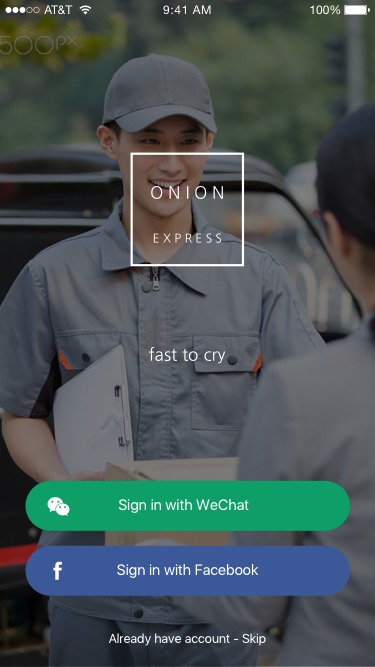
\includegraphics[width=3in]{DocumentRes/Login.png}
  \caption{Log in}
\end{figure}
\begin{figure}[htbp]
  \centering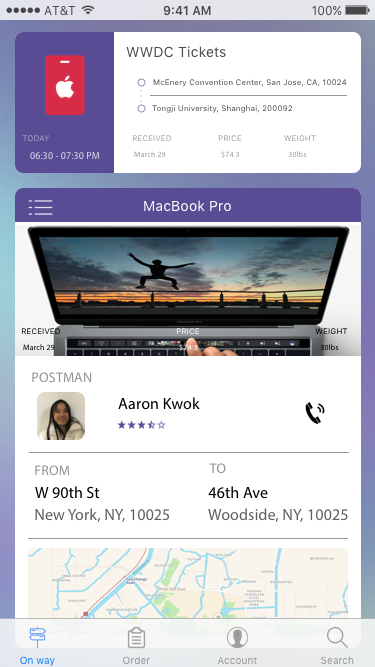
\includegraphics[width=3in]{DocumentRes/OnWay.png}
  \caption{On Way}
\end{figure}
\begin{figure}[htbp]
  \centering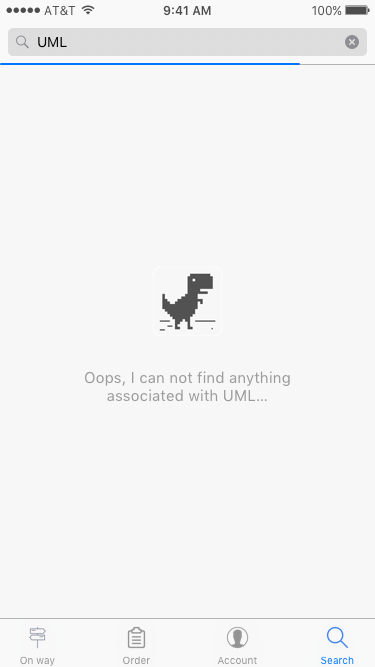
\includegraphics[width=3in]{DocumentRes/Search.png}
  \caption{Search}
\end{figure}
\begin{figure}[htbp]
  \centering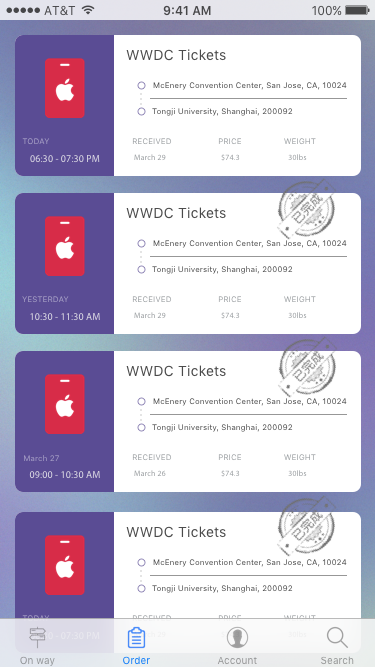
\includegraphics[width=3in]{DocumentRes/Order.png}
  \caption{Order}
\end{figure}
\begin{figure}[htbp]
  \centering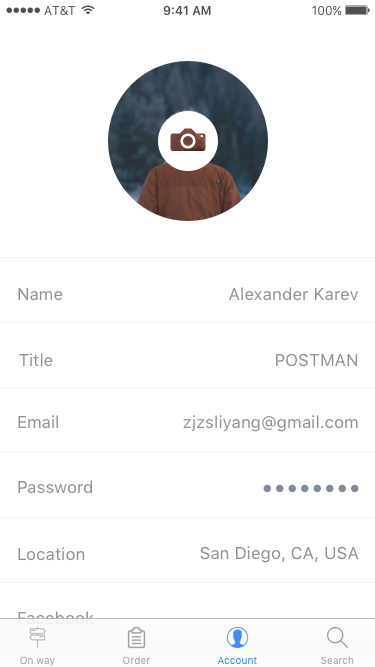
\includegraphics[width=3in]{DocumentRes/Account.png}
  \caption{Account}
\end{figure}

\section{Website}

\chapter{Contributions}
Visit more on \href{https://github.com/zjzsliyang/42003201ObjectOrientedAnalysisAndDesign}{GitHub}
\vspace{3mm}\\
\href{https://github.com/zjzsliyang}{{\color{blue}1452559 Yang LI}} \hspace{17mm} iOS UI, Document\hfill 17\%\\
\href{https://github.com/tjluozhongjin}{{\color{blue}1453645 Zhongjin LUO}} \hspace{5mm} Use Case\hfill 17\%\\
\href{https://github.com/Yghifi}{{\color{blue}1451229 Guohui YANG}} \hspace{4.5mm} Use Case\hfill 17\%\\
\href{https://github.com/Charon0622}{{\color{blue}1552651 Yirui WANG}} \hspace{7mm} Use Case, Activity Diagram, Review\hfill 17\%\\
{{\color{blue}1552677 Xinying WU} \hspace{8mm} Web UI\hfill 17\%\\
\href{https://github.com/lyqun}{{\color{blue}1552705 Yiqun LIN}} \hspace{11mm} Use Case\hfill 17\%

\begin{thebibliography}{99}
\bibitem{1998}
  830-1998,
  \emph{IEEE Recommended Practice for Software Requirements Specifications},
  IEEE,
  Oct 1998.
\bibitem{2011}
  29148-2011,
  \emph{Systems and software engineering -- Life cycle processes --Requirements engineering},
  ISO/IEC/IEEE International Standard,
  Dec 2011.
\bibitem{Miles}
  Russ Miles, Kim Hamilton,
  \emph{Learning UML 2.0},
  O'REILLY,
  1st edtion,
  April 2006.
\bibitem{Arlow}
  Jim Arlow,
  \emph{UML 2.0 and the Unified Process: Practical Object-oriented Analysis and Design},
  ADDISON WESLEY,
  2nd edition,
  2005.
\bibitem{Wiegers}
  Karl Eugene Wiegers, Joy Beatty,
  \emph{Software Requirements},
  Microsoft Press,
  3rd edition,
  2013.
\bibitem{Larman}
  Craig Larman,
  \emph{Applying UML and Patterns},
  Pearson Education International,
  3rd edition,
  2005.
\bibitem{Bennett}
  Simon J. Bennett, Steve McRobb, Ray Farmer,
  \emph{Object-oriented Systems Analysis and Design Using UML},
  McGraw-Hill Education,
  2nd edition,
  Dec 2001.
\bibitem{TAN}
  Yunjie TAN,
  \emph{Thinking in UML},
  China Water Conservancy Hydropower,
  2nd edition,
  March 2012.
\end{thebibliography}

\end{document}
